\documentclass[12pt,a4paper]{standalone}
\usepackage{amssymb}
\usepackage{amsmath}
\usepackage{bm}
\usepackage{tikz}
\usetikzlibrary{arrows.meta}
\usetikzlibrary{arrows}
\usepackage{pstricks}
\usetikzlibrary{patterns}
\usetikzlibrary{fadings}
\usetikzlibrary{shapes.geometric}
\usepackage{ifthen}



\begin{document}
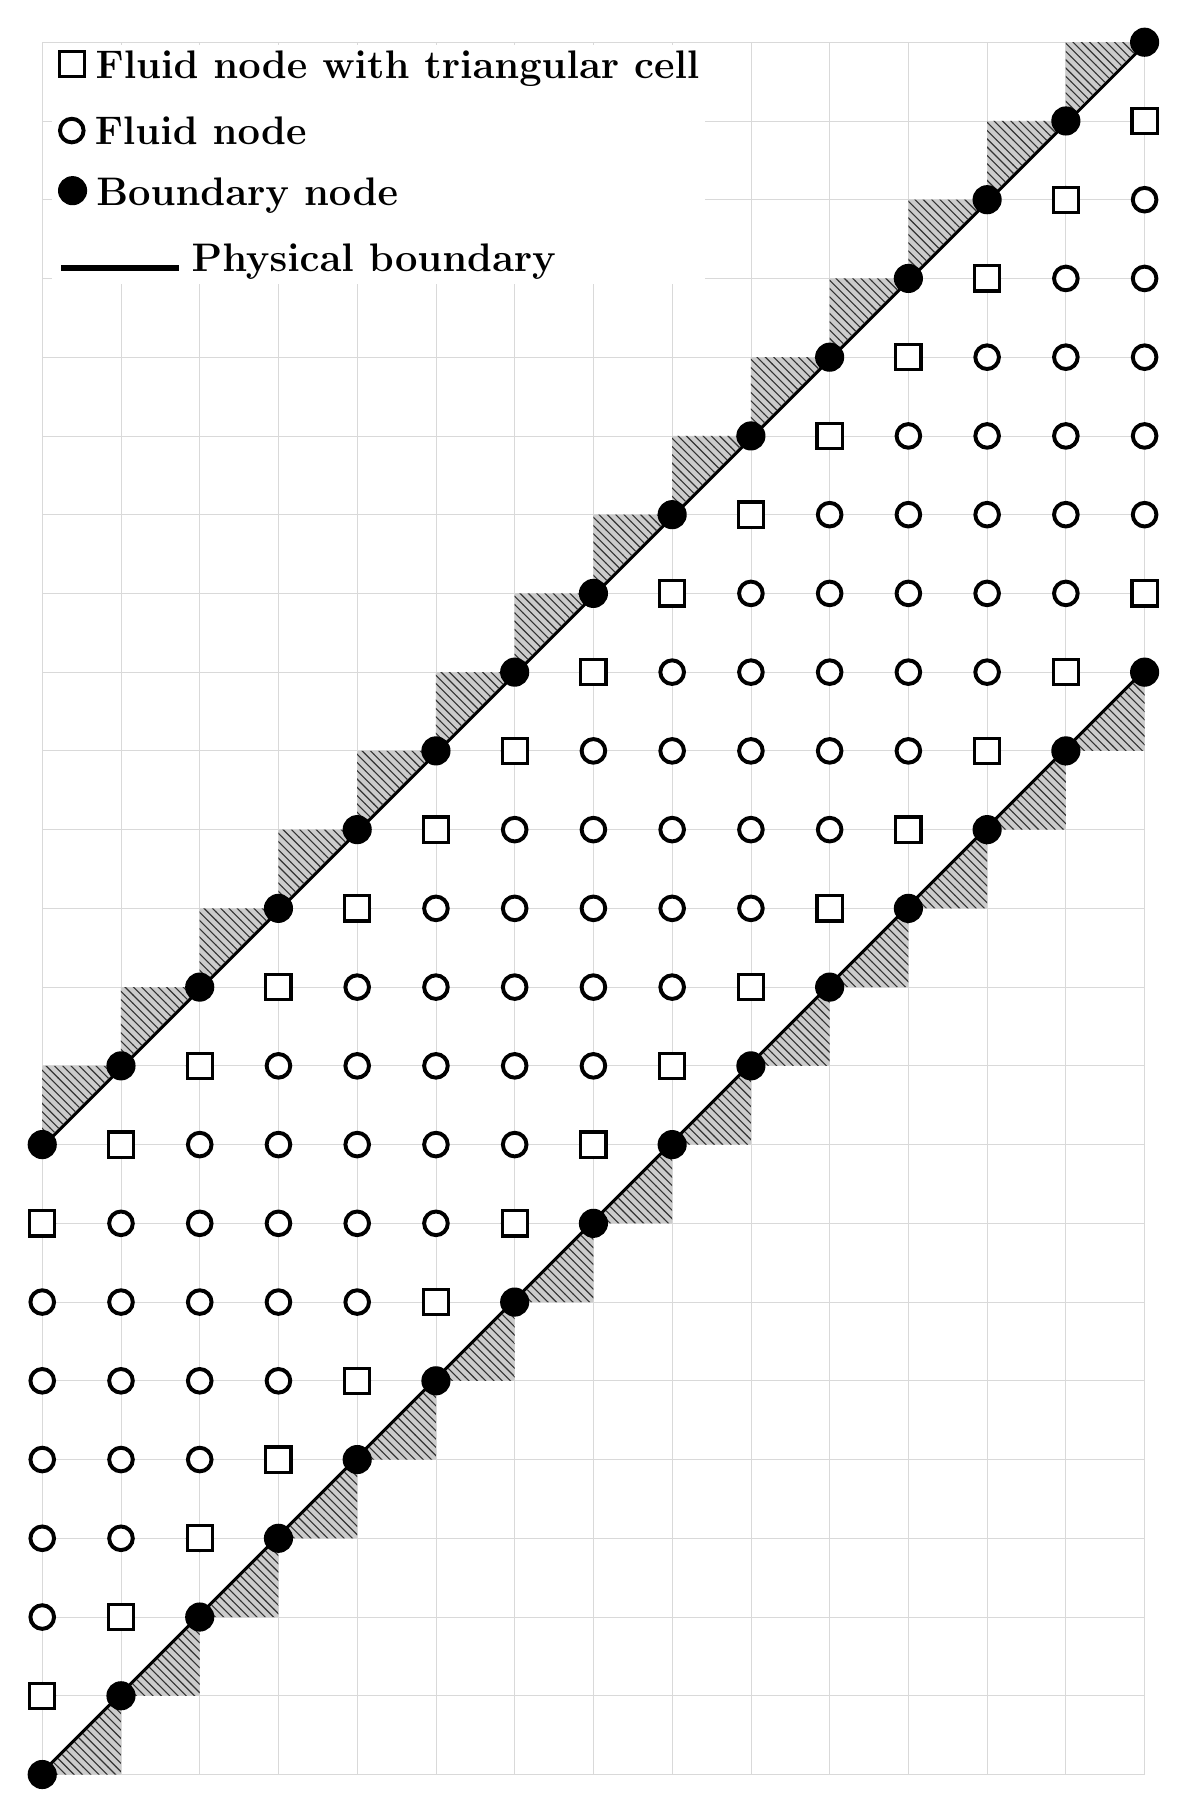
\begin{tikzpicture}[line width=0.6mm]
	

\draw[black, line width=0.8mm] (0,0) -- (14,14);
\draw[black, line width=0.8mm] (0,8) -- (14,22);

\tikzset{myred/.style={draw=black, fill=black, line width=0.2mm, circle, minimum size=0.35cm, inner sep=0pt}}
\tikzset{myblue/.style={draw=black, fill=white, line width=0.5mm, circle, minimum size=0.3cm, inner sep=0pt}}
\tikzset{myblue2/.style={draw=blue, fill=blue, line width=0.5mm, diamond, minimum size=0.45cm, inner sep=0pt}}
\tikzset{mygray/.style={draw=gray!30, fill=gray!30, line width=0.5mm, circle, minimum size=0.25cm, inner sep=0pt}}

\tikzset{
	mysquare/.style={ 
		draw=black,
		fill=white,
		line width=0.4mm,
		rectangle,
		minimum size=0.32cm,
		inner sep=0pt
	}
}


% Horizontal and vertical grid lines
\foreach \y in {0,...,22} {
	\draw[gray!30, line width=0.1mm] (0,\y) -- (14,\y);
}
\foreach \x in {0,...,14} {
	\draw[gray!30, line width=0.1mm] (\x,0) -- (\x,22);
}


\foreach \n in {0,...,13} {
	\fill[black!20]
	(\n,\n) -- (\n+1,\n) -- (\n+1,\n+1) -- cycle;
	\fill[black!20,pattern=north west lines, pattern color=black!80]
	(\n,\n) -- (\n+1,\n) -- (\n+1,\n+1) -- cycle;
%	\fill[pattern=north east lines, pattern color=black!80]
%	(\n,\n) -- (\n+1,\n) -- (\n+1,\n+1) -- cycle;
}

\foreach \n in {0,...,13} {
	\fill[black!20] 	(\n,\n+8) -- (\n,\n+9) -- (\n+1,\n+9) -- cycle;
	\fill[black!20,pattern=north west lines, pattern color=black!80]
	(\n,\n+8) -- (\n,\n+9) -- (\n+1,\n+9) -- cycle;
%	\fill[pattern=north east lines, pattern color=black!80]
%	(\n,\n+8) -- (\n,\n+9) -- (\n+1,\n+9) -- cycle;
}

\fill[black!20] (13,21) -- (13,22) -- (14,22) -- cycle;

\fill[pattern=north west lines, pattern color=black!80]
(13,21) -- (13,22) -- (14,22) -- cycle;

%\fill[pattern=north east lines,  pattern color=black!80]
%(13,21) -- (13,22) -- (14,22) -- cycle;

%%Solid nodes below y=x (bottom line)
%\foreach \x in {0,...,14} {
%	\foreach \y in {0,...,22} {
%		\ifthenelse{\y < \x}{
%			\node[mygray] at (\x,\y) {};
%		}{}
%	}
%}

%%Solid nodes below y=x + 8 (top line)
%\foreach \x in {0,...,14} {
%	\foreach \y in {0,...,22} {
%		\ifthenelse{\y > \numexpr \x + 8\relax}{
%			\node[mygray] at (\x,\y) {};
%		}{}
%	}
%}

%red nodes on y=x (bottom line)
\foreach \x in {0,...,14} {
	\foreach \y in {0,...,22} {
		\ifthenelse{\y = \x}{
			\node[myred] at (\x,\y) {};
		}{}
	}
}

%red nodes on on y=x+8
\foreach \x in {0,...,14} {
	\foreach \y in {0,...,22} {
		\ifthenelse{\y = \numexpr \x + 8\relax}{
			\node[myred] at (\x,\y) {};
		}{}
	}
}

\foreach \x in {0,...,14} {
		\foreach \y in {0,...,22} {
				\ifthenelse{\y > \x \AND \y < \numexpr \x + 8\relax}{
						\node[myblue] at (\x,\y) {};
					}{}
			}
	}

%bc nodes below on y=x+8
\foreach \x in {0,...,14} {
	\foreach \y in {0,...,22} {
		\ifthenelse{\y = \numexpr \x + 7\relax}{
			\node[mysquare] at (\x,\y) {};
		}{}
	}
}

%bc nodes above on y=x+1
\foreach \x in {0,...,14} {
	\foreach \y in {0,...,22} {
		\ifthenelse{\y = \numexpr \x + 1\relax}{
			\node[mysquare] at (\x,\y) {};
		}{}
	}
}


%
%
%\draw (0,25) node[anchor=west] { \tikz{\node[myblue] {};} {\Large\textbf{Fluid node}} };
%\draw (7,25) node[anchor=west] { \tikz{\node[myred] {};} {\Large\textbf{Boundary node}} };
%\draw (0,24) node[anchor=west] { \tikz{\node[mygray] {};} {\Large\textbf{Solid node}} };
%\draw (5.8,24) node[anchor=west] { \tikz{\draw[black,thick, line width=0.8mm] (0,0.8) -- (1.5,0.8);} {\Large\textbf{Physical boundary}} };
%\draw (0,23) node[anchor=west] { \tikz{\node[myblue2] {};} {\Large\textbf{Fluid node with missing neighbour}} };




\node[
line width=0.6mm,
rectangle,
fill=white,
anchor=north west,
align=left,
inner sep=2pt
] at (0.1,22) {%
	\tikz{\node[mysquare] {};} {\Large\textbf{Fluid node with triangular cell}}\\[10pt]
	\tikz{\node[myblue] {};} {\Large\textbf{Fluid node}}\\[10pt]
	\tikz{\node[myred] {};} {\Large\textbf{Boundary node}}\\[10pt]
%	\tikz{\node[mygray] {};} {\Large\textbf{Solid node}}\\[10pt]
	\tikz{\draw[black,line width=0.8mm] (0,0.8)--(1.5,0.8);} {\Large\textbf{Physical boundary}}
};



\end{tikzpicture}



\end{document}



